\documentclass[tikz,border=4pt]{standalone}
\usetikzlibrary{positioning,fit,backgrounds,arrows.meta}

\begin{document}
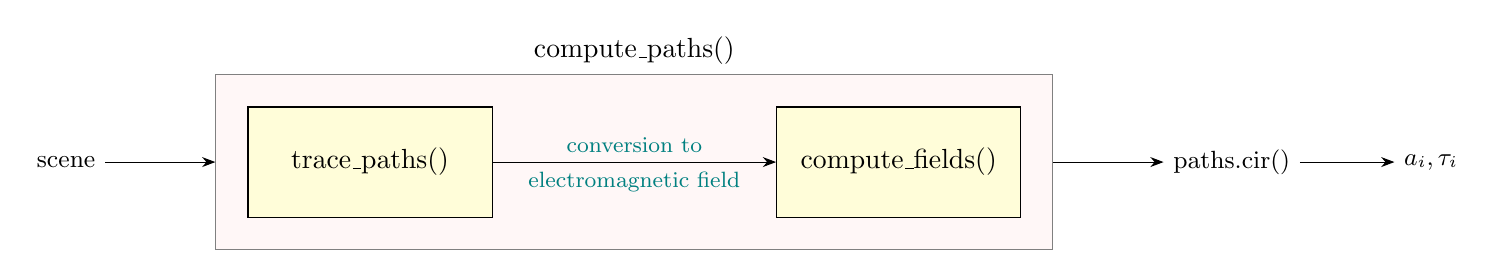
\begin{tikzpicture}[
    node distance=1.1cm and 1.1cm,
    box/.style={rectangle, draw=black, fill=yellow!15, minimum width=3.1cm, minimum height=1.4cm, align=center},
    outerbox/.style={rectangle, draw=gray, fill=red!3, inner sep=0.4cm},
    txt/.style={align=center, font=\small},
    >=Stealth
]
    % blocks
    \node[box] (trace) {trace\_paths()};
    \node[box, right=3.6cm of trace] (fields) {compute\_fields()};

    \begin{scope}[on background layer]
        \node[outerbox, fit=(trace)(fields), label={[align=center]above:compute\_paths()}] (outer) {};
    \end{scope}

    % scene input
    \node[txt, left=1.4cm of outer] (scene) {scene};
    \draw[->] (scene) -- (outer.west |- scene);

    % arrow between trace and fields
    \draw[->] (trace) -- node[txt, midway, above, teal, font=\footnotesize] {conversion to} node[txt, midway, below, teal, font=\footnotesize] {electromagnetic field} (fields);

    % output
    \node[txt, right=1.4cm of outer] (cir) {paths.cir()};
    \draw[->] (outer.east |- cir) -- (cir);

    \node[txt, right=1.2cm of cir] (ai) {$a_i,\tau_i$};
    \draw[->] (cir) -- (ai);
\end{tikzpicture}
\end{document}
